% Graphical Abstract - Journal of Biomedical Informatics
% BioRender-style flat schematic. Compile with pdflatex.
\documentclass[12pt]{article}
\usepackage[margin=0.2in,paperwidth=20cm,paperheight=7cm]{geometry}
\usepackage{tikz}
\usepackage{helvet}
\renewcommand{\familydefault}{\sfdefault}
\usetikzlibrary{arrows.meta,positioning,shapes.geometric}
\pagestyle{empty}

\tikzset{
  pics/person/.style={code={
    \fill[blue!60] (0,0.62) circle (0.30);
    \fill[blue!45] (-0.55,0.05) .. controls (-0.55,-0.60) and (0.55,-0.60) .. (0.55,0.05) -- (-0.55,0.05) -- cycle;
  }},
  pics/doc/.style={code={
    \draw[fill=white, draw=blue!55, rounded corners=2pt, line width=0.8pt] (-0.38,-0.52) rectangle (0.38,0.52);
    \draw[blue!45] (-0.20,0.24) -- (0.20,0.24);
    \draw[blue!45] (-0.20,0.04) -- (0.20,0.04);
    \draw[blue!45] (-0.20,-0.16) -- (0.20,-0.16);
  }},
  pics/checkdoc/.style={code={
    \draw[fill=white, draw=green!60, rounded corners=2pt, line width=0.8pt] (-0.38,-0.52) rectangle (0.38,0.52);
    \draw[green!60, line width=1.1pt] (-0.22,0.08) -- (-0.06,0.26) -- (0.28,-0.24);
  }},
  pics/manifold/.style={code={
    \draw[teal!70!black, thick] (-0.95,0) .. controls (-0.45,0.95) and (0.45,0.95) .. (0.95,0)
      .. controls (0.45,-0.95) and (-0.45,-0.95) .. (-0.95,0);
    \fill[teal!70!black] (-0.55,0.47) circle (1.8pt);
    \fill[teal!70!black] (0.0,0.72) circle (1.8pt);
    \fill[teal!70!black] (0.55,0.47) circle (1.8pt);
    \draw[->, teal!70!black, line width=1pt] (0.0,0.72) -- (0.42,0.82);
  }},
  pics/gate/.style={code={
    \draw[orange!80!black, line width=1pt] (-0.42,-0.55) -- (-0.42,0.55);
    \draw[orange!80!black, line width=1pt] (0.42,-0.55) -- (0.42,0.55);
    \draw[orange!80!black, line width=1pt] (-0.42,0.55) -- (0.42,0.55);
    \draw[rotate around={18:(0.42,-0.55)}, fill=orange!35, draw=orange!80!black, line width=0.8pt]
      (0.42,-0.55) rectangle (0.62,0.55);
    \fill[orange!90!black] (0,0) circle (1.5pt);
  }},
  pics/jepa/.style={code={
    \draw[green!70!black, line width=1.2pt] (0,0) circle (0.46);
    \draw[green!70!black, line width=1pt] (0,0) -- (0,0.16) -- (0.14,0.28);
    \draw[->, green!70!black, line width=1.2pt] (0.45,0.35) -- (0.95,0.35);
    \draw[green!70!black, line width=1pt] (0.62,0.55) -- (0.74,0.55);
  }},
  pics/speed/.style={code={
    \draw[purple!70!black, line width=1.2pt] (0,0) arc (0:180:0.62);
    \draw[purple!70!black, line width=1pt] (-0.62,0) -- (0.62,0);
    \draw[->, purple!70!black, line width=1.5pt] (0,0) -- (-0.28,0.42);
    \fill[purple!70!black] (0,0) circle (2pt);
  }},
  panel/.style={rounded corners=8pt, draw, line width=1.1pt},
  lab/.style={font=\small, text=black!85},
  subtitle/.style={font=\scriptsize, text=black!60},
  arr/.style={-{Stealth[length=4.5mm]}, line width=1.4pt}
}

\begin{document}
\noindent
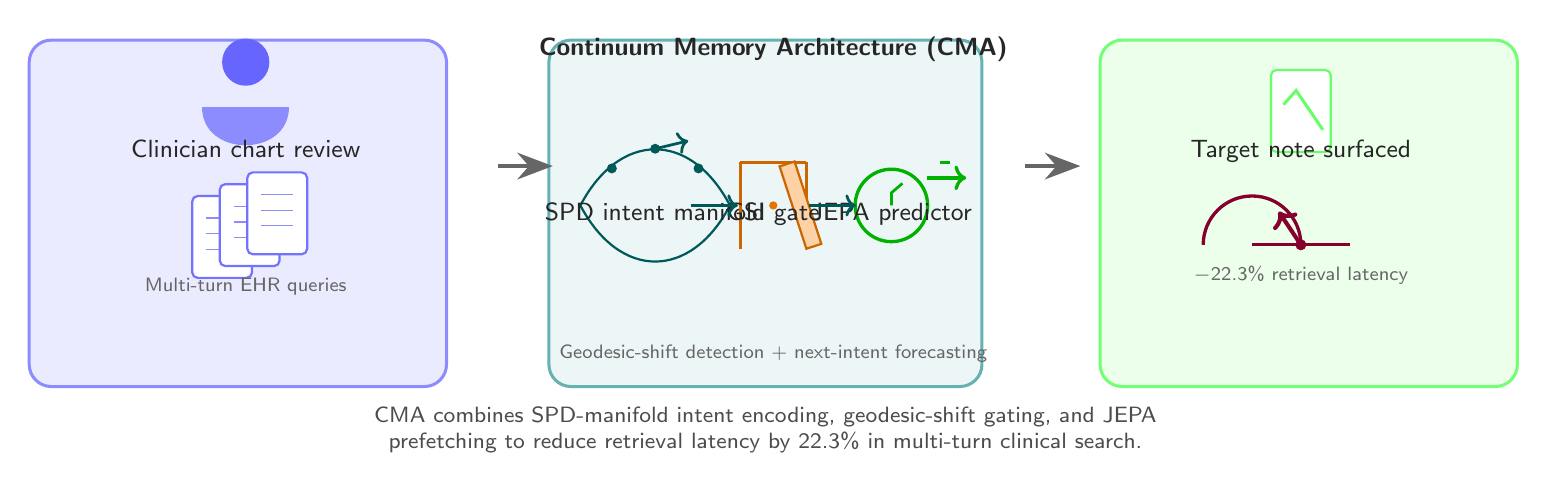
\begin{tikzpicture}[x=1cm,y=1cm]

% ---------------- Panel 1: clinician chart review ----------------
\node[panel, fill=blue!8, draw=blue!45, minimum width=5.3cm, minimum height=4.4cm] (p1) at (3.5,3.3) {};
\draw (3.6,4.6) pic {person};
\node[lab, anchor=north] at (3.6,4.35) {Clinician chart review};
\draw (3.3,3.0) pic {doc};
\draw (3.65,3.15) pic {doc};
\draw (4.0,3.3) pic {doc};
\node[subtitle, anchor=north] at (3.6,2.6) {Multi-turn EHR queries};

% ---------------- Panel 2: CMA ----------------
\node[panel, fill=teal!7, draw=teal!60, minimum width=5.5cm, minimum height=4.4cm] (p2) at (10.2,3.3) {};
\node[lab, font=\small\bfseries, anchor=south] at (10.3,5.1) {Continuum Memory Architecture (CMA)};

\draw (8.8,3.4) pic {manifold};
\node[lab, anchor=north] at (8.8,3.55) {SPD intent manifold};
\draw (10.3,3.4) pic {gate};
\node[lab, anchor=north] at (10.3,3.55) {GSI gate};
\draw (11.8,3.4) pic {jepa};
\node[lab, anchor=north] at (11.8,3.55) {JEPA predictor};

\draw[->, teal!70!black, line width=1pt] (9.25,3.4) -- (9.85,3.4);
\draw[->, teal!70!black, line width=1pt] (10.75,3.4) -- (11.35,3.4);

\node[subtitle, anchor=north] at (10.3,1.75) {Geodesic-shift detection + next-intent forecasting};

% ---------------- Panel 3: results ----------------
\node[panel, fill=green!8, draw=green!55, minimum width=5.3cm, minimum height=4.4cm] (p3) at (17.1,3.3) {};
\draw (17.0,4.6) pic {checkdoc};
\node[lab, anchor=north] at (17.0,4.35) {Target note surfaced};
\draw (17.0,2.9) pic {speed};
\node[subtitle, anchor=north] at (17.0,2.75) {$-$22.3\% retrieval latency};

% ---------------- Inter-panel arrows ----------------
\draw[arr, color=black!60] (6.8,3.9) -- (7.5,3.9);
\draw[arr, color=black!60] (13.5,3.9) -- (14.2,3.9);

% ---------------- Caption ----------------
\node[font=\footnotesize, text=black!70, text width=16cm, align=center] at (10.2,0.55)
  {CMA combines SPD-manifold intent encoding, geodesic-shift gating, and JEPA prefetching to reduce retrieval latency by 22.3\% in multi-turn clinical search.};

\end{tikzpicture}
\end{document}
